\documentclass[aspectratio=169,10pt,t]{beamer}

% -----------------------------------------------------------------------------
% Overleaf-safe packages (pdfLaTeX)
% -----------------------------------------------------------------------------
\usepackage[T1]{fontenc}
\usepackage{lmodern}
\usepackage{amsmath,amssymb,bm}
\usepackage{booktabs,tabularx,array,colortbl}
\usepackage{graphicx}
\usepackage{tikz}
\usetikzlibrary{arrows.meta,positioning,calc,fit,shapes.geometric}

% -----------------------------------------------------------------------------
% Editable title metadata
% -----------------------------------------------------------------------------
\newcommand{\PresenterName}{Zhang Rongchuan}
\newcommand{\PresenterAffiliation}{Institute for Artificial Intelligence}
\newcommand{\TalkVenue}{Master Thesis}
\newcommand{\TitleLineOne}{Relation-Conditioned Row-Graph}
\newcommand{\TitleLineTwo}{Learning for Relational Prediction}

\title[Relation-Conditioned Row Graphs]{\TitleLineOne\ \TitleLineTwo}
\author{\PresenterName}
\institute{\PresenterAffiliation}
\date{\TalkVenue}

% -----------------------------------------------------------------------------
% Visual identity
% -----------------------------------------------------------------------------
\definecolor{Navy}{HTML}{19324A}
\definecolor{Blue}{HTML}{376A9E}
\definecolor{Teal}{HTML}{247A73}
\definecolor{Purple}{HTML}{7461A8}
\definecolor{Orange}{HTML}{B8611C}
\definecolor{Red}{HTML}{B94A48}
\definecolor{Green}{HTML}{327A61}
\definecolor{Ink}{HTML}{223047}
\definecolor{Muted}{HTML}{66758A}
\definecolor{PaleBlue}{HTML}{EEF4F9}
\definecolor{PalePurple}{HTML}{F3F0F8}
\definecolor{PaleOrange}{HTML}{FBF1E7}
\definecolor{PaleTeal}{HTML}{EAF5F3}
\definecolor{PaleRed}{HTML}{F8ECEB}
\definecolor{Line}{HTML}{D5DEE8}

\renewcommand{\familydefault}{\sfdefault}
\usefonttheme{professionalfonts}
\setbeamercolor{normal text}{fg=Ink,bg=white}
\setbeamercolor{structure}{fg=Navy}
\setbeamercolor{frametitle}{fg=Navy,bg=white}
\setbeamerfont{frametitle}{series=\bfseries,size=\large}
\setbeamerfont{title}{series=\bfseries}
\setbeamerfont{subtitle}{size=\normalsize}
\setbeamerfont{block title}{series=\bfseries,size=\normalsize}
\setbeamerfont{block body}{size=\small}
\setbeamerfont{block title alerted}{series=\bfseries,size=\normalsize}
\setbeamerfont{block body alerted}{size=\small}
\setbeamerfont{block title example}{series=\bfseries,size=\normalsize}
\setbeamerfont{block body example}{size=\small}
\setbeamerfont{footline}{size=\fontsize{5.8}{6.6}\selectfont}
\setbeamertemplate{navigation symbols}{}
\setbeamersize{text margin left=0.72cm,text margin right=0.72cm}
\setbeamertemplate{blocks}[rounded][shadow=false]

\setbeamertemplate{frametitle}{%
  \vspace*{.34cm}% fixed top breathing room
  \hspace*{.72cm}%
  \begin{minipage}{\dimexpr\paperwidth-1.44cm\relax}
    \raggedright
    \usebeamerfont{frametitle}%
    \usebeamercolor[fg]{frametitle}%
    \strut\insertframetitle\strut\par
    \vspace{.10cm}% title-to-rule spacing
    {\color{Line}\rule{\linewidth}{.55pt}}%
  \end{minipage}%
  \par\vspace{.16cm}% rule-to-content spacing
}

\setbeamertemplate{footline}{%
  \leavevmode
  \hbox{%
    \begin{beamercolorbox}[wd=.78\paperwidth,ht=2.7ex,dp=1.05ex,leftskip=.72cm]{author in head/foot}%
      \color{Muted}\insertshorttitle
    \end{beamercolorbox}%
    \begin{beamercolorbox}[wd=.22\paperwidth,ht=2.7ex,dp=1.05ex,rightskip=.72cm plus1fil]{date in head/foot}%
      \hfill\color{Muted}\insertframenumber\,/\,\inserttotalframenumber
    \end{beamercolorbox}%
  }
}

\setbeamertemplate{itemize item}{\color{Orange}$\blacktriangleright$}
\setbeamertemplate{itemize subitem}{\color{Teal}$\bullet$}
\setlength{\leftmargini}{1.15em}
\setlength{\leftmarginii}{1.2em}

\newcommand{\source}[1]{\vfill\par{\fontsize{6.3}{7.2}\selectfont\color{Muted}Source: #1}}
\newcommand{\metric}[1]{{\bfseries\color{Navy}#1}}
\newcommand{\good}[1]{{\bfseries\color{Green}#1}}
\newcommand{\bad}[1]{{\bfseries\color{Red}#1}}
\newcommand{\keyeq}[1]{%
  \begin{beamercolorbox}[sep=.45em,wd=\linewidth]{block body}
    \centering #1
  \end{beamercolorbox}}

\setbeamercolor{block title}{fg=white,bg=Navy}
\setbeamercolor{block body}{fg=Ink,bg=PaleBlue}
\setbeamercolor{block title alerted}{fg=white,bg=Orange}
\setbeamercolor{block body alerted}{fg=Ink,bg=PaleOrange}
\setbeamercolor{block title example}{fg=white,bg=Teal}
\setbeamercolor{block body example}{fg=Ink,bg=PaleTeal}
\setbeamercolor{author in head/foot}{fg=Muted,bg=white}
\setbeamercolor{date in head/foot}{fg=Muted,bg=white}
\setbeamercolor{GapOneTitle}{fg=white,bg=Orange}
\setbeamercolor{GapOneBody}{fg=Ink,bg=PaleOrange}
\setbeamercolor{GapTwoTitle}{fg=white,bg=Blue}
\setbeamercolor{GapTwoBody}{fg=Ink,bg=PaleBlue}
\setbeamercolor{GapThreeTitle}{fg=white,bg=Teal}
\setbeamercolor{GapThreeBody}{fg=Ink,bg=PaleTeal}

\newcommand{\contentcard}[4]{%
  \begin{beamercolorbox}[wd=\linewidth,sep=.12cm,leftskip=.04cm,rightskip=.04cm]{#1}
    \strut\bfseries #3\strut
  \end{beamercolorbox}%
  \begin{beamercolorbox}[wd=\linewidth,sep=.16cm]{#2}
    \small\raggedright
    \hyphenpenalty=10000\exhyphenpenalty=10000
    #4\par
  \end{beamercolorbox}%
}

\AtBeginDocument{%
  \setlength{\abovedisplayskip}{.45em}%
  \setlength{\belowdisplayskip}{.45em}%
  \setlength{\abovedisplayshortskip}{.3em}%
  \setlength{\belowdisplayshortskip}{.3em}%
}

\tikzset{
  row/.style={draw=Blue,fill=PaleBlue,rounded corners=2pt,minimum width=1.65cm,minimum height=.72cm,align=center,font=\small\bfseries},
  rel/.style={draw=Purple,fill=PalePurple,rounded corners=2pt,minimum width=2.05cm,minimum height=.72cm,align=center,font=\small\bfseries},
  cand/.style={draw=Orange,fill=PaleOrange,diamond,aspect=1.5,inner sep=2.5pt,align=center,font=\small\bfseries},
  seed/.style={draw=Orange,fill=PaleOrange,rounded corners=2pt,minimum width=1.75cm,minimum height=.78cm,align=center,font=\small\bfseries},
  fk/.style={-{Stealth[length=2mm]},draw=Blue,line width=.9pt},
  rev/.style={-{Stealth[length=2mm]},draw=Teal,line width=.9pt},
  cond/.style={-{Stealth[length=2mm]},draw=Orange,dashed,line width=1pt},
}

\begin{document}

% -----------------------------------------------------------------------------
% 1. Title
% -----------------------------------------------------------------------------
\begin{frame}[plain]
  \begin{tikzpicture}[remember picture,overlay]
    \fill[Navy] (current page.north west) rectangle ([yshift=-.68cm]current page.north east);
    \fill[PaleBlue] ([yshift=.72cm]current page.south west) rectangle (current page.south east);
    \fill[Orange] ([xshift=.82cm,yshift=.34cm]current page.south west) rectangle ([xshift=3.15cm,yshift=.39cm]current page.south west);

    \node[circle,fill=Purple,minimum size=.25cm] (rtop) at ([xshift=-1.58cm,yshift=-.27cm]current page.north east) {};
    \node[circle,fill=Teal,minimum size=.17cm] (rbot) at ([xshift=-1.12cm,yshift=-.48cm]current page.north east) {};
    \draw[Purple,line width=1.05pt] (rtop) -- (rbot);

    \node[anchor=north west,text width=14.1cm,align=left,inner sep=0pt]
      at ([xshift=.82cm,yshift=-1.20cm]current page.north west) {%
        {\fontsize{21}{24}\selectfont\bfseries\color{Navy}
        \TitleLineOne\\[-.02cm]\TitleLineTwo}%
      };

    \node[anchor=north west,text width=13.8cm,align=left,inner sep=0pt]
      at ([xshift=.84cm,yshift=-3.08cm]current page.north west)
      {{\fontsize{11.5}{13.5}\selectfont\color{Orange}\insertsubtitle}};

    \draw[Line,line width=.6pt]
      ([xshift=.82cm,yshift=-3.53cm]current page.north west) --
      ([xshift=8.05cm,yshift=-3.53cm]current page.north west);

    \node[anchor=north west,inner sep=0pt]
      at ([xshift=.82cm,yshift=-3.87cm]current page.north west)
      {{\fontsize{12.5}{14.5}\selectfont\bfseries\color{Navy}\PresenterName}};

    \node[anchor=north west,inner sep=0pt,align=left]
      at ([xshift=.82cm,yshift=-4.34cm]current page.north west)
      {{\fontsize{9.5}{11.5}\selectfont\color{Muted}
        \PresenterAffiliation\hspace{.25cm}%
        {\color{Line}\rule{.7pt}{.82em}}\hspace{.25cm}%
        \TalkVenue}};
  \end{tikzpicture}
\end{frame}

% -----------------------------------------------------------------------------
% 2. Problem definition，three limitations of current relational prediction
% -----------------------------------------------------------------------------
\begin{frame}{Three limitations of current relational prediction}
  \vspace{.12cm}
  \begin{columns}[T,onlytextwidth]
    \column{.32\textwidth}
      \vspace{0pt}
      \contentcard{GapOneTitle}{GapOneBody}
        {1. Shortcut dependence}
        {RT predictions depend strongly on historical target labels from the same entity.}
    \column{.32\textwidth}
      \vspace{0pt}
      \contentcard{GapTwoTitle}{GapTwoBody}
        {2. Coarse FK relations}
        {RT encodes FK direction, but not an explicit table-pair type: Results $\rightarrow$ Drivers and Results $\rightarrow$ Races are both $\mathsf{f2p}$.}
  \end{columns}

  % \vspace{.50cm}
  % \begin{beamercolorbox}[sep=.62em,wd=\linewidth]{block body}
  %   \centering
  %   \normalsize\bfseries
  %   Can we retain predictive accuracy while making the relational path explicit, compact, and less dependent on self-label shortcuts?
  % \end{beamercolorbox}
\end{frame}

% -----------------------------------------------------------------------------
% 3. NSL validation protocol
% -----------------------------------------------------------------------------
\begin{frame}{Validation protocol: No-Self-Label (NSL)}
  \small
  Both settings mask the seed target and evaluate the same checkpoint on the same test queries.
  Standard may retain a sampled self-label; NSL skips every sampled self-label.

  \vspace{.10cm}
  \begin{columns}[T,onlytextwidth]
    \column{.47\textwidth}
      \vspace{0pt}
      \begin{block}{Standard context}
        \centering
        \renewcommand{\arraystretch}{1.08}
        \setlength{\tabcolsep}{5pt}
        \begin{tabular}{lrr}
          \toprule
          Time & driverId & DNF label \\
          \midrule
          \rowcolor{PaleOrange}$t$ & 10 & \texttt{MASK} \\
          $t-1$ & 10 & \cellcolor{PaleRed}{\color{Red}\bfseries 1} \\
          $t-2$ & 10 & \cellcolor{PaleRed}{\color{Red}\bfseries 0} \\
          $t-1$ & 47 & 1 \\
          \bottomrule
        \end{tabular}

        \vspace{.08cm}
        \raggedright\scriptsize
        A sampled same-entity target value may remain visible.
      \end{block}

    \column{.47\textwidth}
      \vspace{0pt}
      \begin{alertblock}{NSL context}
        \centering
        \renewcommand{\arraystretch}{1.08}
        \setlength{\tabcolsep}{5pt}
        \begin{tabular}{lrr}
          \toprule
          Time & driverId & DNF label \\
          \midrule
          \rowcolor{PaleOrange}$t$ & 10 & \texttt{MASK} \\
          $t-1$ & 10 & \cellcolor{PaleRed}{\color{Red}\bfseries skipped} \\
          $t-2$ & 10 & \cellcolor{PaleRed}{\color{Red}\bfseries skipped} \\
          $t-1$ & 47 & 1 \\
          \bottomrule
        \end{tabular}

        \vspace{.08cm}
        \raggedright\scriptsize
        Every sampled same-entity target value is skipped.
      \end{alertblock}
  \end{columns}

  \vspace{.10cm}
  \begin{beamercolorbox}[sep=.34em,wd=\linewidth]{block body}
    \centering
    \textbf{NSL drop} $=$ \textbf{Standard score} $-$ \textbf{NSL score}
  \end{beamercolorbox}

\end{frame}


% -----------------------------------------------------------------------------
% 4. Classification evidence
% -----------------------------------------------------------------------------
\begin{frame}{Classification evidence: local RT drops 17.8 points under NSL}
  \begin{columns}[T,onlytextwidth]
    \column{.38\textwidth}
      \vspace{0pt}
      \begin{block}{Paired macro average}
        \centering
        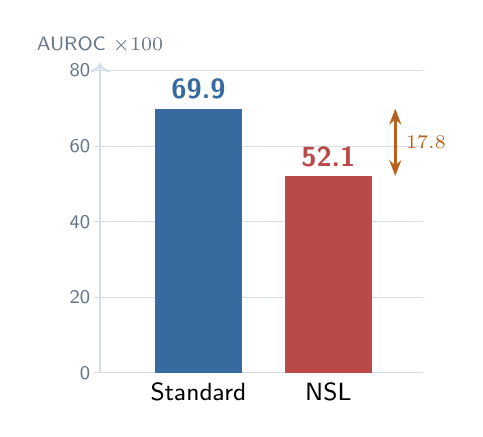
\begin{tikzpicture}[x=1cm,y=.048cm]
          \draw[->,Line,line width=.8pt] (0,0) -- (0,82) node[above,font=\scriptsize,Muted] {AUROC $\times100$};
          \foreach \y in {0,20,40,60,80}{
            \draw[Line] (-.08,\y) -- (4.1,\y);
            \node[left,font=\scriptsize,Muted] at (0,\y) {\y};
          }
          \fill[Blue] (.7,0) rectangle (1.8,69.9);
          \fill[Red] (2.35,0) rectangle (3.45,52.1);
          \node[above,font=\bfseries,Blue] at (1.25,69.9) {69.9};
          \node[above,font=\bfseries,Red] at (2.9,52.1) {52.1};
          \node[below,font=\small] at (1.25,0) {Standard};
          \node[below,font=\small] at (2.9,0) {NSL};
          \draw[{Stealth[length=2mm]}-{Stealth[length=2mm]},Orange,line width=1.2pt] (3.75,52.1) -- node[right,font=\scriptsize\bfseries,Orange] {$17.8$} (3.75,69.9);
        \end{tikzpicture}
      \end{block}

    \column{.58\textwidth}
      \vspace{0pt}
      \begin{block}{All 10 paired classification tasks}
        \fontsize{6.7}{7.7}\selectfont
        \renewcommand{\arraystretch}{1.08}
        \setlength{\tabcolsep}{2.7pt}
        \begin{tabularx}{\linewidth}{Xrrr}
          \toprule
          Task & Std. & NSL & Drop $\downarrow$ \\
          \midrule
          Amazon Item Churn & 70.2 & 51.8 & {\color{Red}18.4} \\
          Amazon User Churn & 64.6 & 54.9 & {\color{Red}9.7} \\
          Avito User Clicks & 58.5 & 53.9 & {\color{Red}4.6} \\
          Avito User Visits & 62.1 & 48.0 & {\color{Red}14.2} \\
          F1 Driver DNF & 79.1 & 69.7 & {\color{Red}9.4} \\
          F1 Driver Top-3 & 89.1 & 46.3 & \bad{42.8} \\
          H\&M User Churn & 64.2 & 39.6 & \bad{24.6} \\
          Stack User Badge & 80.6 & 54.3 & \bad{26.3} \\
          Stack User Engagement & 78.3 & 49.9 & \bad{28.4} \\
          Trial Study Outcome & 52.4 & 52.4 & 0.0 \\
          \bottomrule
        \end{tabularx}
      \end{block}
  \end{columns}
  \source{Local paired full-test evaluation of the released RT checkpoints. Drop is Standard minus NSL and is computed before rounding; each pair uses the same checkpoint and test queries.}
\end{frame}


% -----------------------------------------------------------------------------
% 5. Design answer
% -----------------------------------------------------------------------------
\begin{frame}{Design principles: from cells to rows and relations}
  \vspace{.15cm}
  \centering
  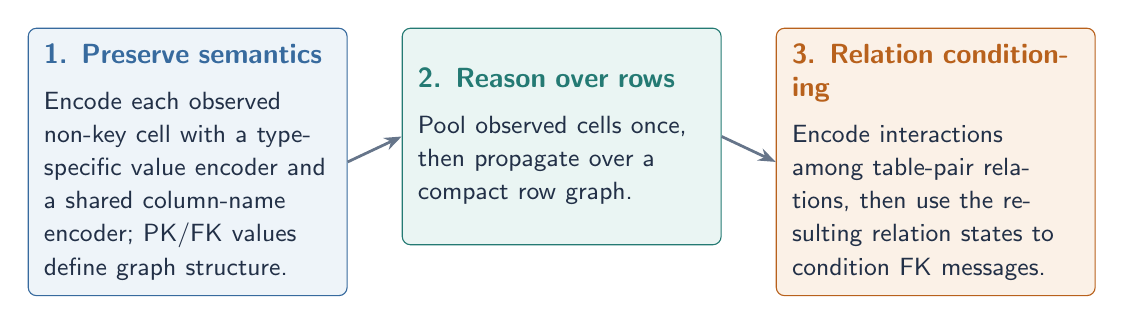
\begin{tikzpicture}
    \node[anchor=north,draw=Blue,fill=PaleBlue,rounded corners=3pt,
          text width=3.65cm,minimum height=2.75cm,inner sep=.20cm,align=left] (p1) at (-4.75,0) {%
      {\bfseries\color{Blue}1. Preserve semantics}\\[.16cm]
      {\small\color{Ink}Encode each observed non-key cell with a type-specific value encoder and a shared column-name encoder; PK/FK values define graph structure.}};
    \node[anchor=north,draw=Teal,fill=PaleTeal,rounded corners=3pt,
          text width=3.65cm,minimum height=2.75cm,inner sep=.20cm,align=left] (p2) at (0,0) {%
      {\bfseries\color{Teal}2. Reason over rows}\\[.16cm]
      {\small\color{Ink}Pool observed cells once, then propagate over a compact row graph.}};
    \node[anchor=north,draw=Orange,fill=PaleOrange,rounded corners=3pt,
          text width=3.65cm,minimum height=2.75cm,inner sep=.20cm,align=left] (p3) at (4.75,0) {%
      {\bfseries\color{Orange}3. Relation conditioning}\\[.16cm]
      {\small\color{Ink}Encode interactions among table-pair relations, then use the resulting relation states to condition FK messages.}};
    \draw[-{Stealth[length=2.2mm]},Muted,line width=1pt] (p1.east) -- (p2.west);
    \draw[-{Stealth[length=2.2mm]},Muted,line width=1pt] (p2.east) -- (p3.west);

  \end{tikzpicture}
\end{frame}

% -----------------------------------------------------------------------------
% 6. Base architecture
% -----------------------------------------------------------------------------
\begin{frame}{RowGraph-Base Architecture}
  \centering
  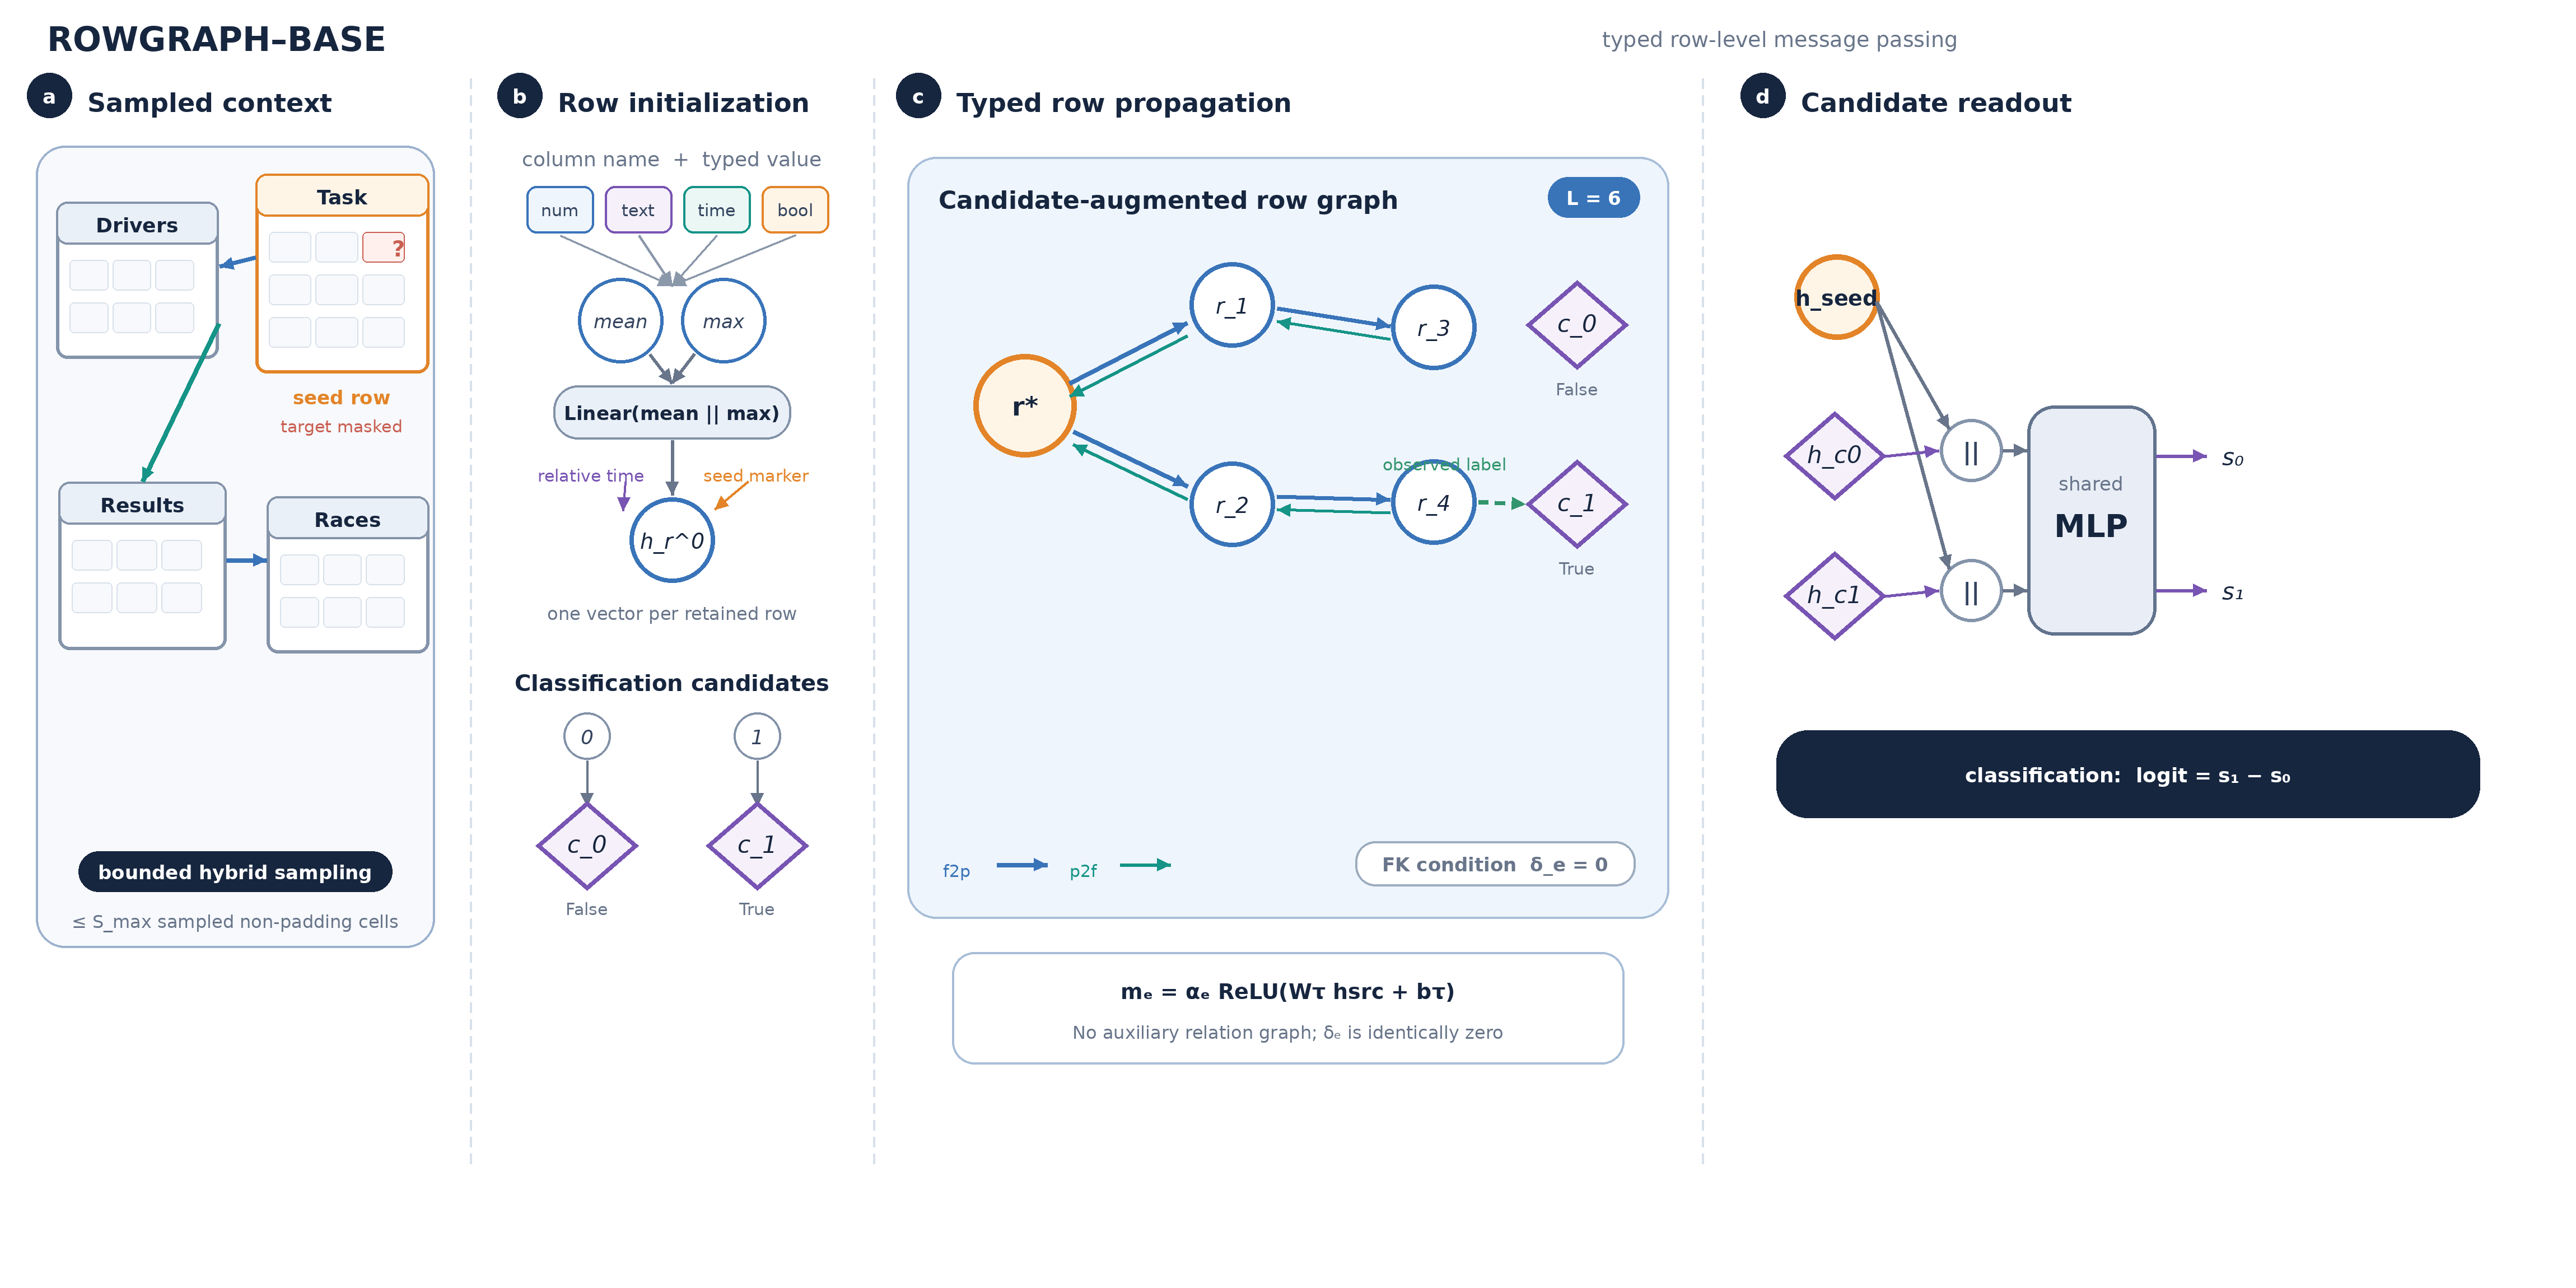
\includegraphics[width=.95\linewidth]{figures/rowgraph_base_architecture.png}
\end{frame}

% -----------------------------------------------------------------------------
% 7. RelGraph architecture
% -----------------------------------------------------------------------------
\begin{frame}{RelGraph Architecture}
  \centering
  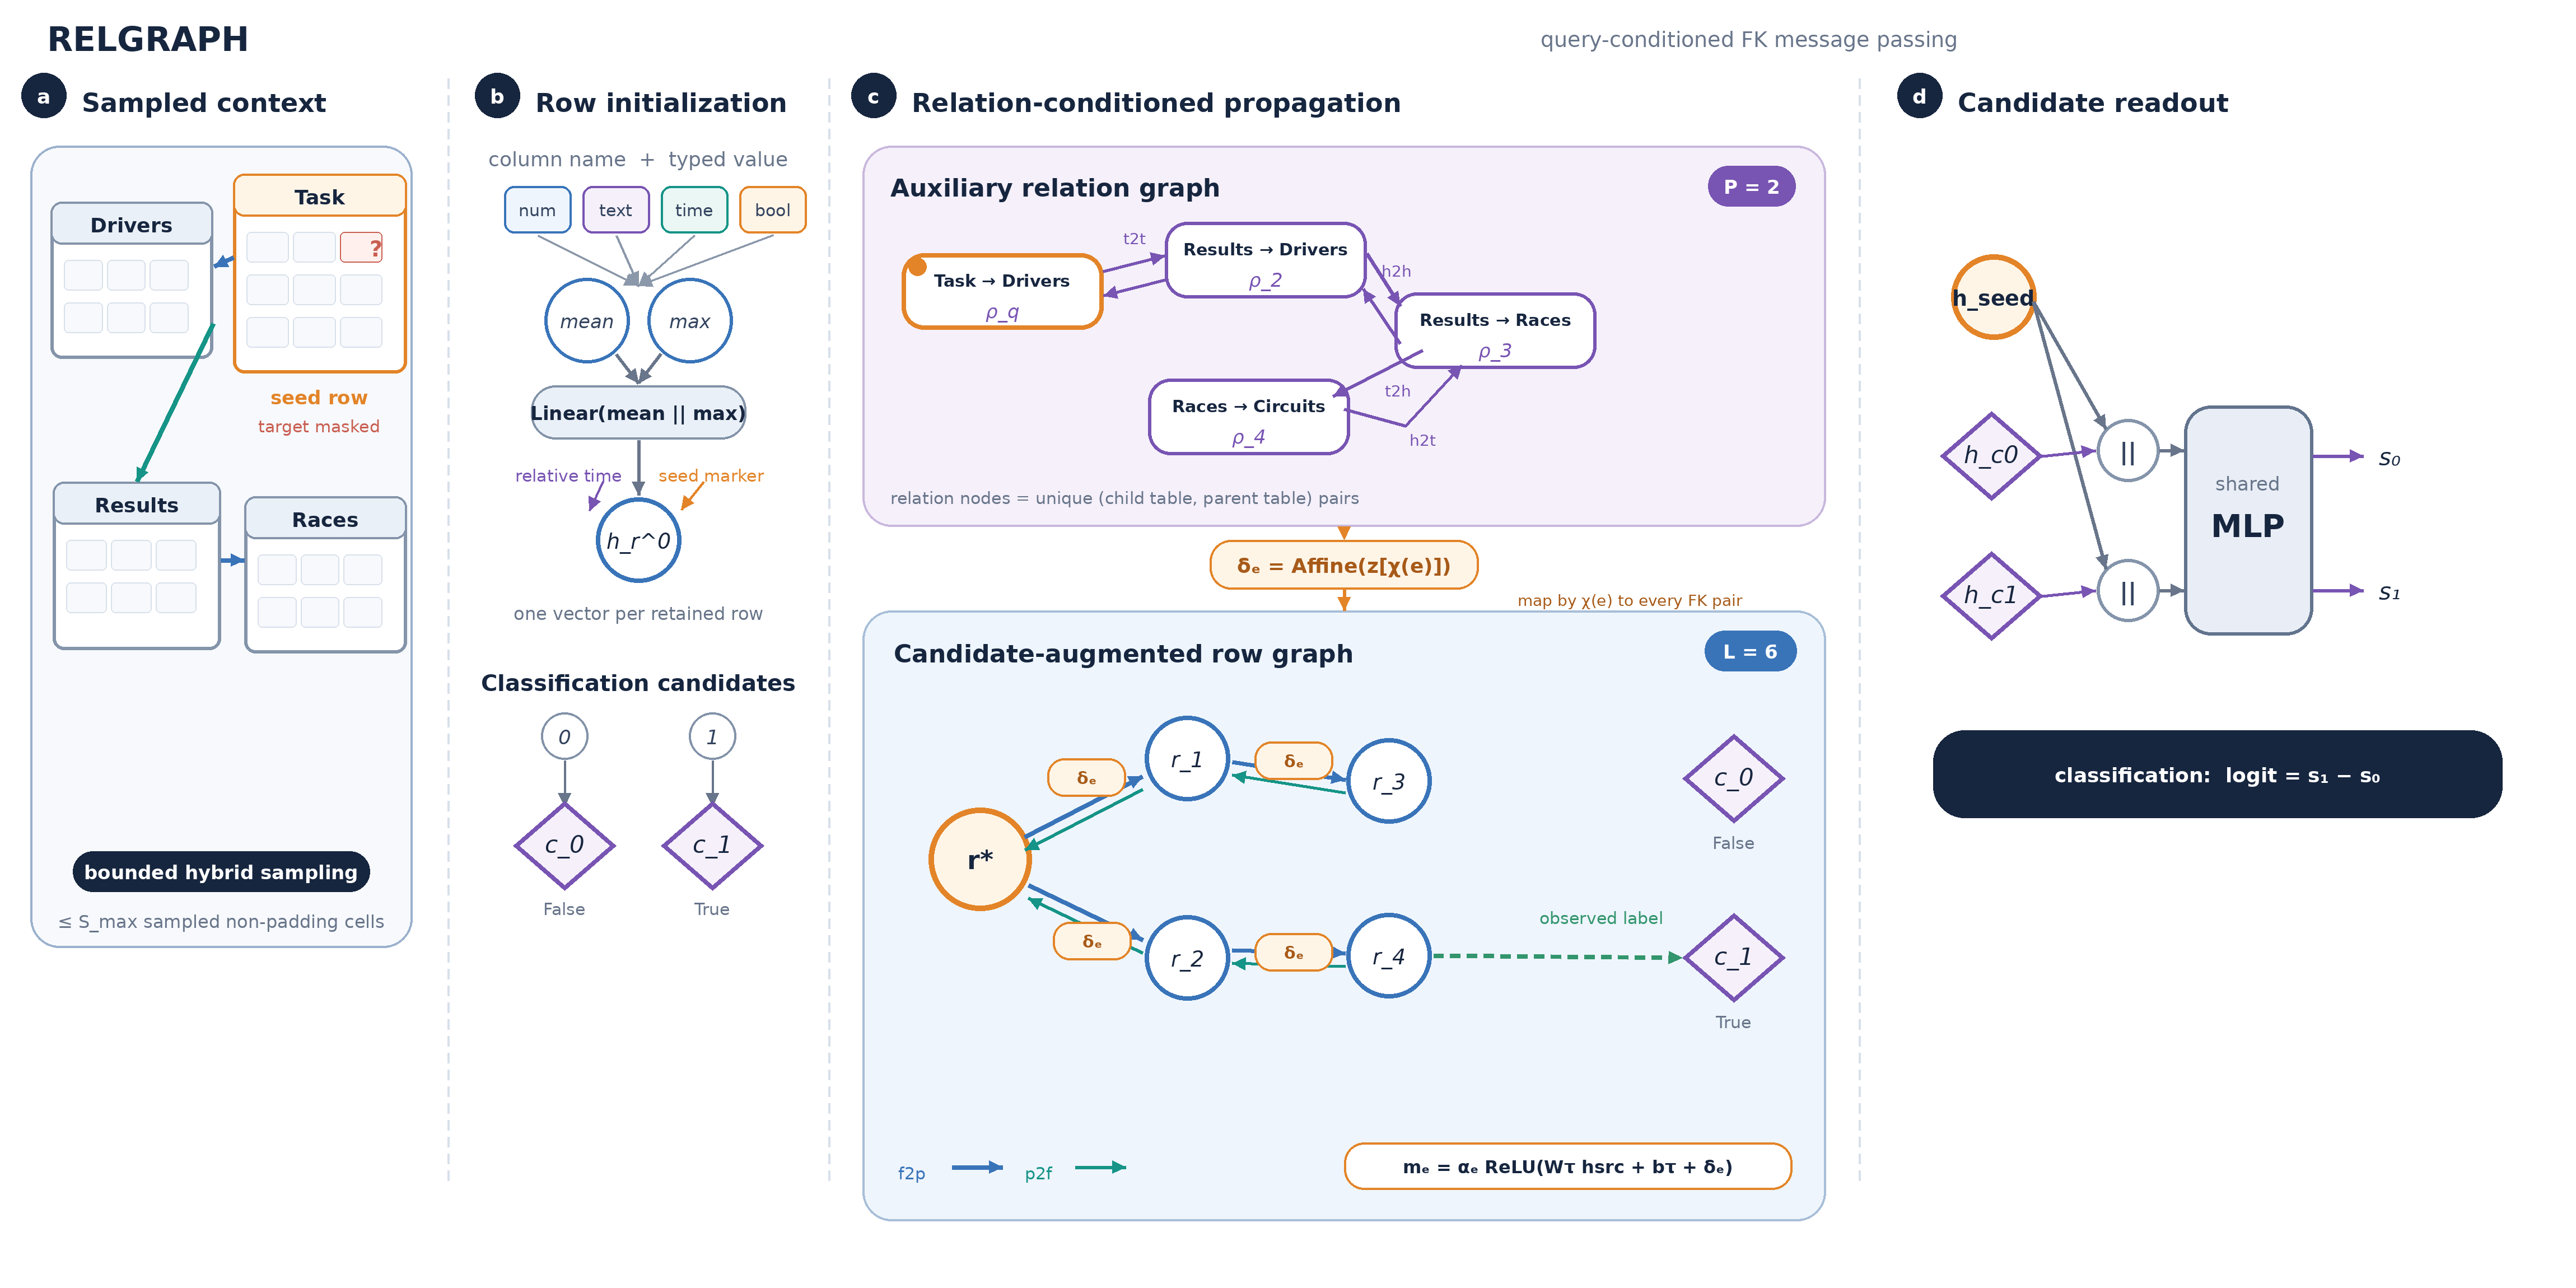
\includegraphics[width=.95\linewidth]{figures/relgraph_architecture.png}
\end{frame}

% -----------------------------------------------------------------------------
% 8. Sampler detail
% -----------------------------------------------------------------------------
\begin{frame}{Seed-centered relational context sampling}
  \begin{columns}[T,onlytextwidth]
    \column{.51\textwidth}
      \vspace{0pt}
      \centering
      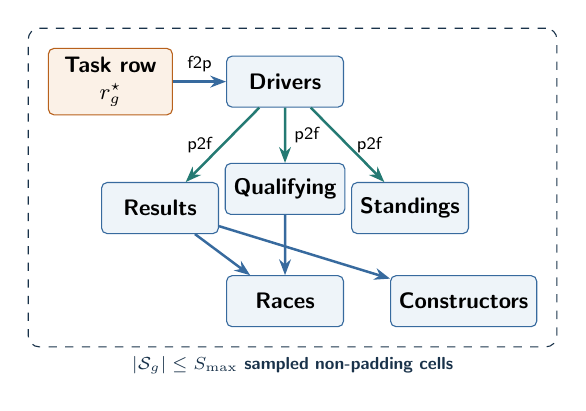
\begin{tikzpicture}[node distance=.65cm and .75cm,scale=.9,transform shape]
        \node[seed] (task) {Task row\\$r_g^\star$};
        \node[row,right=of task] (driver) {Drivers};
        \node[row,below left=1.05cm and .1cm of driver] (results) {Results};
        \node[row,below=.78cm of driver] (qual) {Qualifying};
        \node[row,below right=1.05cm and .1cm of driver] (stand) {Standings};
        \node[row,below=.85cm of qual] (races) {Races};
        \node[row,right=.65cm of races] (construct) {Constructors};
        \draw[fk] (task) -- node[above,font=\scriptsize] {$\mathsf{f2p}$} (driver);
        \draw[rev] (driver) -- node[left,font=\scriptsize] {$\mathsf{p2f}$} (results);
        \draw[rev] (driver) -- node[right,font=\scriptsize] {$\mathsf{p2f}$} (qual);
        \draw[rev] (driver) -- node[right,font=\scriptsize] {$\mathsf{p2f}$} (stand);
        \draw[fk] (results) -- (races);
        \draw[fk] (qual) -- (races);
        \draw[fk] (results) -- (construct);
        \node[draw=Navy,dashed,rounded corners,fit=(task)(driver)(results)(stand)(races)(construct),inner sep=.25cm,label={[font=\scriptsize\bfseries,text=Navy]below:$|\mathcal S_g|\le S_{\max}$ sampled non-padding cells}] {};
      \end{tikzpicture}

    \column{.45\textwidth}
      \vspace{0pt}
      \keyeq{%
        \small
        $\mathcal S_g=\operatorname{Sample}\!(
          \mathcal G^{\mathrm{DB}},r_g^\star;S_{\max},B_{\max})$}
      \vspace{.2cm}
      \small
      \begin{itemize}
        \item Traverse both $\mathsf{f2p}$ and $\mathsf{p2f}$ links; serialize each visited row at most once.
        \item Prioritize $\mathsf{f2p}$ with a LIFO frontier; otherwise randomize $\mathsf{p2f}$ neighbors at the shallowest pending depth.
        \item $S_{\max}=2048$ counts serialized cells, not rows; the final row may contribute only a prefix.
        \item Cap each reverse-FK expansion at $B_{\max}=256$ randomly selected database children; for forecasting, discard a child later than the seed when both timestamps are present.
      \end{itemize}
  \end{columns}
\end{frame}


% % -----------------------------------------------------------------------------
% % 9. Sampling example: context coverage regression
% % -----------------------------------------------------------------------------
% \begin{frame}{Sampling example I: from one driver query to relational context}
%   \vspace{.02cm}
%   \begin{columns}[c,onlytextwidth]
%     \column{.30\textwidth}
%       \begin{alertblock}{Seed task row}
%         \centering
%         {\fontsize{7.2}{8.2}\selectfont
%         \setlength{\tabcolsep}{3.2pt}
%         \renewcommand{\arraystretch}{1.25}
%         \begin{tabular}{ccc}
%           \toprule
%           \textbf{date} & \textbf{driverId} & \textbf{position} \\
%           \midrule
%           2004-07-05 & \bfseries 10 & \color{Red}\bfseries MASK \\
%           \bottomrule
%         \end{tabular}}

%         \vspace{.20cm}
%         {\scriptsize Held-out target for evaluation: \textbf{10.75}}
%       \end{alertblock}

%       \vspace{.18cm}
%       \begin{beamercolorbox}[sep=.58em,wd=\linewidth]{block body}
%         \small
%         \textbf{driverId $=10$} anchors the FK traversal; the seed target value is never exposed to the model.
%       \end{beamercolorbox}

%     \column{.08\textwidth}
%       \centering
%       \begin{tikzpicture}
%         \draw[-{Stealth[length=3mm]},Blue,line width=1.7pt] (0,0) -- (.82,0);
%         \node[font=\fontsize{5.8}{6.5}\selectfont,text=Muted,align=center] at (.41,.38) {bounded FK\\traversal};
%       \end{tikzpicture}

%     \column{.58\textwidth}
%       \begin{block}{Reachable context in this diagnostic}
%         \centering
%         {\fontsize{6.75}{7.45}\selectfont
%         \setlength{\tabcolsep}{4.2pt}
%         \renewcommand{\arraystretch}{1.06}
%         \begin{tabularx}{\linewidth}{>{\raggedright\arraybackslash}X r r r}
%           \rowcolor{Navy}
%           \color{white}\bfseries Table &
%           \color{white}\bfseries Rows &
%           \color{white}\bfseries Columns &
%           \color{white}\bfseries Cells \\
%           task table                    & 15  & 3  & 45   \\
%           \rowcolor{PaleBlue}drivers    & 1   & 7  & 7    \\
%           results                       & 28  & 15 & 420  \\
%           \rowcolor{PaleBlue}qualifying & 13  & 7  & 91   \\
%           standings                     & 27  & 7  & 189  \\
%           \rowcolor{PaleBlue}races      & 28  & 7  & 196  \\
%           constructors                  & 2   & 4  & 8    \\
%           \rowcolor{PaleBlue}constructor\_results & 316 & 5 & 1580 \\
%           constructor\_standings        & 304 & 7  & 2128 \\
%           \rowcolor{PaleBlue}circuits   & 18  & 8  & 144  \\
%           \rowcolor{PaleOrange}
%           \bfseries Total               & \bfseries 752 & \bfseries 70 & \bfseries 4808 \\
%         \end{tabularx}}
%       \end{block}
%   \end{columns}

%   \vspace{.13cm}
%   \begin{beamercolorbox}[sep=.52em,wd=\linewidth]{block body}
%     \centering\small
%     The reachable context is larger than the budget, so the sampler retains a bounded prefix:
%     \textbf{$S_{\max}=1024$ cells in this illustration}; the main experiments use \textbf{$S_{\max}=2048$}.
%   \end{beamercolorbox}
% \end{frame}

% % -----------------------------------------------------------------------------
% % 10. Sampling example: traversal and serialization regression
% % -----------------------------------------------------------------------------
% \begin{frame}{Sampling example II: FK traversal and the cell budget}
%   \vspace{.02cm}
%   \begin{columns}[T,onlytextwidth]
%     \column{.44\textwidth}
%       \begin{block}{Query-centered FK traversal}
%         \centering
%         \begin{tikzpicture}[x=1cm,y=1cm,scale=.70,transform shape]
%           \node[seed,minimum width=2.85cm] (task) at (0,4.55) {Task row\\\scriptsize driverId $=10$};
%           \node[row,minimum width=2.25cm] (drivers) at (0,3.30) {Drivers\\\scriptsize driverId $=10$};
%           \node[row,minimum width=1.55cm] (results) at (-2.25,1.80) {Results};
%           \node[row,minimum width=1.70cm] (qual) at (0,1.80) {Qualifying};
%           \node[row,minimum width=1.65cm] (stand) at (2.25,1.80) {Standings};
%           \node[row,minimum width=1.55cm] (races) at (-.65,.38) {Races};
%           \node[row,minimum width=1.75cm] (circuits) at (-1.75,-.95) {Circuits};
%           \node[row,minimum width=2.10cm] (construct) at (1.20,-.95) {Constructors};
%           \node[row,minimum width=2.20cm,font=\scriptsize\bfseries] (cres) at (.10,-2.35) {Constructor\\Results};
%           \node[row,minimum width=2.20cm,font=\scriptsize\bfseries] (cstand) at (2.55,-2.35) {Constructor\\Standings};

%           \draw[fk] (task) -- node[right,font=\tiny] {driverId: $\mathsf{f2p}$} (drivers);
%           \draw[rev] (drivers) -- node[left,font=\tiny] {$\mathsf{p2f}$} (results);
%           \draw[rev] (drivers) -- node[right,font=\tiny] {$\mathsf{p2f}$} (qual);
%           \draw[rev] (drivers) -- node[right,font=\tiny] {$\mathsf{p2f}$} (stand);
%           \draw[fk] (results) -- node[left,font=\tiny] {raceId} (races);
%           \draw[fk] (qual) -- (races);
%           \draw[fk] (stand) -- (races);
%           \draw[fk] (races) -- node[left,font=\tiny] {circuitId} (circuits);
%           \draw[fk] (results.south east) to[bend right=11] (construct.north west);
%           \draw[fk] (qual.south east) to[bend left=10] node[right,font=\tiny] {constructorId} (construct.north);
%           \draw[rev] (construct) -- (cres);
%           \draw[rev] (construct) -- node[right,font=\tiny] {$\mathsf{p2f}$} (cstand);
%         \end{tikzpicture}

%         \vspace{-.08cm}
%         {\fontsize{6.2}{7}\selectfont
%           \color{Blue}$\longrightarrow$ foreign-to-primary ($\mathsf{f2p}$)
%           \hspace{.55em}
%           \color{Teal}$\longrightarrow$ primary-to-foreign ($\mathsf{p2f}$)}
%       \end{block}

%     \column{.52\textwidth}
%       \begin{block}{Retained cells: long-format excerpt}
%         \centering
%         {\fontsize{5.65}{6.45}\selectfont
%         \setlength{\tabcolsep}{2.15pt}
%         \renewcommand{\arraystretch}{1.22}
%         \begin{tabularx}{\linewidth}{r >{\raggedright\arraybackslash}X r l >{\raggedleft\arraybackslash}p{1.52cm}}
%           \rowcolor{Navy}
%           \color{white}\bfseries Cell &
%           \color{white}\bfseries Table &
%           \color{white}\bfseries Raw row &
%           \color{white}\bfseries Column &
%           \color{white}\bfseries Value \\
%           0    & task table & 642  & date & 2002-08-15 \\
%           \rowcolor{PaleBlue}1 & task table & 695  & date & 2002-09-14 \\
%           2    & task table & 1338 & date & 2002-05-17 \\
%           \rowcolor{PaleBlue}3 & task table & 1340 & date & 2002-06-16 \\
%           4    & task table & 1342 & date & 2002-07-16 \\
%           \multicolumn{5}{c}{\color{Muted}$\vdots$} \\
%           1019 & constructor\_results & 6661 & constructorResultsId & 6661 \\
%           \rowcolor{PaleBlue}1020 & constructor\_results & 6667 & constructorResultsId & 6667 \\
%           1021 & constructor\_results & 6680 & constructorResultsId & 6680 \\
%           \rowcolor{PaleBlue}1022 & constructor\_results & 6703 & constructorResultsId & 6703 \\
%           1023 & constructor\_results & 6713 & constructorResultsId & 6713 \\
%         \end{tabularx}}
%       \end{block}
%   \end{columns}

%   \vspace{.12cm}
%   \begin{beamercolorbox}[sep=.52em,wd=\linewidth]{block body}
%     \centering\small
%     \textbf{1024 long-format records $=$ 1024 sampled cells, not 1024 database rows.}
%     Visited database rows are admitted cell by cell, and the final retained row may contribute only a prefix of its cells.
%   \end{beamercolorbox}
% \end{frame}

% -----------------------------------------------------------------------------
% 9. Sampling example: eligible relational neighborhood classification
% -----------------------------------------------------------------------------
\begin{frame}{Sampling example I: expanding from one driver query}
  \vspace{.02cm}
  \begin{columns}[c,onlytextwidth]
    \column{.34\textwidth}
      \begin{alertblock}{Seed task row}
        \centering
        {\fontsize{6.9}{8.0}\selectfont
        \setlength{\tabcolsep}{2.6pt}
        \renewcommand{\arraystretch}{1.25}
        \begin{tabular}{ccc}
          \toprule
          \textbf{date} & \textbf{driverId} & \textbf{did\_not\_finish} \\
          \midrule
          2004-07-05 & \bfseries 10 & \color{Red}\bfseries MASK \\
          \bottomrule
        \end{tabular}}
      \end{alertblock}

      \vspace{.18cm}
      \begin{beamercolorbox}[sep=.58em,wd=\linewidth]{block body}
        \small
        \texttt{driverId}$=10$ is an FK used to traverse the database graph.
        The masked target may occupy a position in $\mathcal S_g$, but never enters $\mathcal C_g^{\mathrm{in}}$.
      \end{beamercolorbox}

    \column{.08\textwidth}
      \centering
      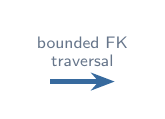
\begin{tikzpicture}
        \draw[-{Stealth[length=3mm]},Blue,line width=1.7pt] (0,0) -- (.82,0);
        \node[font=\fontsize{5.8}{6.5}\selectfont,text=Muted,align=center] at (.41,.38) {bounded FK\\traversal};
      \end{tikzpicture}

    \column{.54\textwidth}
      \begin{block}{Rows made eligible by FK traversal}
        {\small
        \renewcommand{\arraystretch}{1.22}
        \setlength{\tabcolsep}{4pt}
        \begin{tabularx}{\linewidth}{>{\bfseries}l X}
          \toprule
          Expansion & Matching database rows \\
          \midrule
          $\mathsf{f2p}$
            & The \texttt{Drivers} row whose primary key is $10$. \\
          \rowcolor{PaleBlue}
          $\mathsf{p2f}$
            & \texttt{Results}, \texttt{Qualifying}, and \texttt{Standings} rows whose \texttt{driverId} is $10$. \\
          $\mathsf{f2p}$
            & Referenced \texttt{Races} and \texttt{Constructors} rows. \\
          \rowcolor{PaleBlue}
          further FK
            & For example, \texttt{Races} $\rightarrow$ \texttt{Circuits}. \\
          \bottomrule
        \end{tabularx}}
      \end{block}
  \end{columns}

  \vspace{.13cm}
  \begin{beamercolorbox}[sep=.52em,wd=\linewidth]{block body}
    \centering\small
    These rows are \textbf{eligible context}, not a guarantee that all of them fit.
    The priority traversal and the \textbf{$S_{\max}=2048$-cell budget} determine the retained prefix.
  \end{beamercolorbox}
\end{frame}

% -----------------------------------------------------------------------------
% 10. Sampling example: traversal and serialization classification
% -----------------------------------------------------------------------------
\begin{frame}{Sampling example II: FK traversal and the cell budget}
  \vspace{.02cm}
  \begin{columns}[T,onlytextwidth]
    \column{.44\textwidth}
      \begin{block}{Query-centered FK traversal}
        \centering
        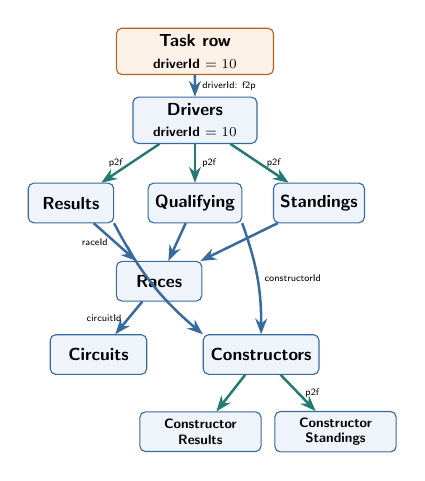
\begin{tikzpicture}[x=1cm,y=1cm,scale=.70,transform shape]
          \node[seed,minimum width=2.85cm] (task) at (0,4.55) {Task row\\\scriptsize driverId $=10$};
          \node[row,minimum width=2.25cm] (drivers) at (0,3.30) {Drivers\\\scriptsize driverId $=10$};
          \node[row,minimum width=1.55cm] (results) at (-2.25,1.80) {Results};
          \node[row,minimum width=1.70cm] (qual) at (0,1.80) {Qualifying};
          \node[row,minimum width=1.65cm] (stand) at (2.25,1.80) {Standings};
          \node[row,minimum width=1.55cm] (races) at (-.65,.38) {Races};
          \node[row,minimum width=1.75cm] (circuits) at (-1.75,-.95) {Circuits};
          \node[row,minimum width=2.10cm] (construct) at (1.20,-.95) {Constructors};
          \node[row,minimum width=2.20cm,font=\scriptsize\bfseries] (cres) at (.10,-2.35) {Constructor\\Results};
          \node[row,minimum width=2.20cm,font=\scriptsize\bfseries] (cstand) at (2.55,-2.35) {Constructor\\Standings};

          \draw[fk] (task) -- node[right,font=\tiny] {driverId: $\mathsf{f2p}$} (drivers);
          \draw[rev] (drivers) -- node[left,font=\tiny] {$\mathsf{p2f}$} (results);
          \draw[rev] (drivers) -- node[right,font=\tiny] {$\mathsf{p2f}$} (qual);
          \draw[rev] (drivers) -- node[right,font=\tiny] {$\mathsf{p2f}$} (stand);
          \draw[fk] (results) -- node[left,font=\tiny] {raceId} (races);
          \draw[fk] (qual) -- (races);
          \draw[fk] (stand) -- (races);
          \draw[fk] (races) -- node[left,font=\tiny] {circuitId} (circuits);
          \draw[fk] (results.south east) to[bend right=11] (construct.north west);
          \draw[fk] (qual.south east) to[bend left=10] node[right,font=\tiny] {constructorId} (construct.north);
          \draw[rev] (construct) -- (cres);
          \draw[rev] (construct) -- node[right,font=\tiny] {$\mathsf{p2f}$} (cstand);
        \end{tikzpicture}

        \vspace{-.08cm}
        {\fontsize{6.2}{7}\selectfont
          \color{Blue}$\longrightarrow$ foreign-to-primary ($\mathsf{f2p}$)
          \hspace{.55em}
          \color{Teal}$\longrightarrow$ primary-to-foreign ($\mathsf{p2f}$)}
      \end{block}

    \column{.52\textwidth}
      \begin{block}{Row-by-row serialization (schematic)}
        \centering
        {\fontsize{6.2}{7.2}\selectfont
        \setlength{\tabcolsep}{3.0pt}
        \renewcommand{\arraystretch}{1.24}
        \begin{tabularx}{\linewidth}{r l X}
          \toprule
          Order & Retained row & Cells appended to $\mathcal S_g$ \\
          \midrule
          1 & seed task row
            & date; masked DNF target \\
          \rowcolor{PaleBlue}
          2 & \texttt{Drivers}
            & forename; surname; date of birth; nationality; $\ldots$ \\
          3 & one \texttt{Results} row
            & number; grid; position; points; laps; $\ldots$ \\
          \rowcolor{PaleBlue}
          4 & referenced \texttt{Races}
            & year; round; name; date; $\ldots$ \\
          $\vdots$ & $\vdots$ & $\vdots$ \\
          last & retained row
            & only a prefix if the cell budget is exhausted \\
          \bottomrule
        \end{tabularx}}

        \vspace{.12cm}
        \raggedright\scriptsize
        PK values are skipped; FK values create graph edges; null cells contribute no value token.
      \end{block}
  \end{columns}

  \vspace{.12cm}
  \begin{beamercolorbox}[sep=.52em,wd=\linewidth]{block body}
    \centering\small
    $|\mathcal S_g|\le 2048$ counts serialized non-padding cells, whereas
    $\mathcal C_g^{\mathrm{in}}=\{n\in\mathcal S_g:n\text{ is not masked}\}$ is supplied to cell encoding and row pooling.
  \end{beamercolorbox}
\end{frame}
% -----------------------------------------------------------------------------
% 11. Cell encoding and pooling
% -----------------------------------------------------------------------------
\begin{frame}{From heterogeneous cells to row representations}
  \begin{columns}[T,onlytextwidth]
    \column{.47\textwidth}
      \vspace{0pt}
      \begin{block}{Type-aware cell encoding}
        For observed cell $n$ in row $r$:
        \[
          \mathbf x_{r,n}
          =g_{\mathrm{col}}(\mathbf u_{r,n}^{\mathrm{col}})
          +f_{\sigma_{r,n}}(\mathbf u_{r,n}^{\mathrm{val}}).
        \]
        $g_{\mathrm{col}}$ is one shared column-name encoder;
        $f_{\sigma}$ is type specific for
        $\sigma\in\{\mathsf{num},\mathsf{text},\mathsf{datetime},\mathsf{bool}\}$.
        Each encoder is affine followed by RMSNorm.
      \end{block}

    \column{.47\textwidth}
      \vspace{0pt}
      \begin{exampleblock}{Cell-to-row pooling}
        For visible cells $\mathcal O_{g,r}$ in row $r$:
        \[
        \begin{aligned}
          \bm\mu_{g,r} &= \operatorname{mean}_{n\in\mathcal O_{g,r}}\mathbf x_{r,n},\\
          \mathbf m_{g,r} &= \operatorname{max}_{n\in\mathcal O_{g,r}}\mathbf x_{r,n},\\
          \bar{\mathbf h}_{g,r} &= W_{\mathrm{c2r}}[\bm\mu_{g,r}\Vert\mathbf m_{g,r}]+\mathbf b_{\mathrm{c2r}}.
        \end{aligned}
        \]
      \end{exampleblock}
  \end{columns}

  \vspace{.18cm}
  \begin{beamercolorbox}[sep=.55em,wd=\linewidth]{block body}
    \centering\small
    $\mathbf h_{g,r}^{(0)}=\bar{\mathbf h}_{g,r}
    +W_{\mathrm{time}}\bm\phi_{\mathrm{time}}(\Delta t_{g,r})+\mathbf b_{\mathrm{time}}
    +\mathbb{1}[r=r_g^\star]\mathbf e_{\mathrm{seed}}$.
    
    The masked target is excluded before encoding and pooling.
  \end{beamercolorbox}
\end{frame}

% -----------------------------------------------------------------------------
% 12. Candidate-augmented row graph
% -----------------------------------------------------------------------------
\begin{frame}{Candidate-augmented row graph}
  \begin{columns}[T,onlytextwidth]
    \column{.54\textwidth}
      \vspace{0pt}
      \centering
      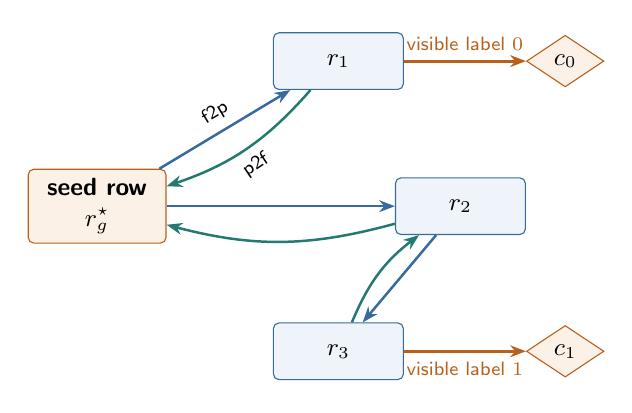
\begin{tikzpicture}[node distance=.75cm and 1.05cm]
        \node[seed] (seed) {seed row\\$r_g^\star$};
        \node[row,above right=1.0cm and 1.35cm of seed] (r1) {$r_1$};
        \node[row,right=2.9cm of seed] (r2) {$r_2$};
        \node[row,below right=1.0cm and 1.35cm of seed] (r3) {$r_3$};
        \node[cand,right=1.55cm of r1] (c0) {$c_0$};
        \node[cand,right=1.55cm of r3] (c1) {$c_1$};
        \draw[fk] (seed) -- node[above,sloped,font=\scriptsize] {$\mathsf{f2p}$} (r1);
        \draw[rev] (r1) to[bend left=15] node[below,sloped,font=\scriptsize] {$\mathsf{p2f}$} (seed);
        \draw[fk] (seed) -- (r2);
        \draw[rev] (r2) to[bend left=15] (seed);
        \draw[fk] (r2) -- (r3);
        \draw[rev] (r3) to[bend left=15] (r2);
        \draw[-{Stealth[length=2mm]},Orange,line width=1.1pt] (r1) -- node[above,font=\scriptsize] {visible label $0$} (c0);
        \draw[-{Stealth[length=2mm]},Orange,line width=1.1pt] (r3) -- node[below,font=\scriptsize] {visible label $1$} (c1);
      \end{tikzpicture}

    \column{.42\textwidth}
      \vspace{0pt}
      \begin{itemize}
        \item One node for each retained row.
        \item Two classification candidate nodes: $c_0$ and $c_1$.
        \item Every retained FK link becomes paired directed $\mathsf{f2p}$/$\mathsf{p2f}$ edges.
        \item A visible historical label creates a \emph{one-way} row-to-candidate edge.
        \item Candidate nodes only receive messages. They never send messages back to row nodes, so candidate-label information cannot alter the encoded context.
      \end{itemize}
  \end{columns}
\end{frame}

% -----------------------------------------------------------------------------
% 13. Base forward
% -----------------------------------------------------------------------------
\begin{frame}{RowGraph-Base message passing}
  \begin{columns}[T,onlytextwidth]
    \column{.52\textwidth}
      \vspace{0pt}
      \begin{block}{Typed edge message}
        For $e:j\rightarrow i$ at layer $\ell$:
        \[
        \setlength{\jot}{.18em}
        \begin{aligned}
          \mathbf q_e^{(\ell)}
          &=W_{\tau_e}^{(\ell)}\mathbf h_j^{(\ell-1)}
            +\mathbf b_{\tau_e}^{(\ell)}
            +\underbrace{\bm\delta_e}_{\mathbf 0\ \text{in Base}},\\
          \mathbf m_e^{(\ell)}
          &=\alpha_e\,\operatorname{ReLU}(\mathbf q_e^{(\ell)}).
        \end{aligned}
        \]
      \end{block}
      \vspace{-.06cm}
      \begin{exampleblock}{Node update}
        \[
        \setlength{\jot}{.18em}
        \begin{aligned}
          \mathbf a_i^{(\ell)}
          &=\frac{\sum_{e\in\mathcal E^-(i)}\mathbf m_e^{(\ell)}}
          {\max(1,\sum_{e\in\mathcal E^-(i)}\alpha_e)},\\
          \mathbf u_i^{(\ell)}
          &=\operatorname{ReLU}\!\left(
            W_{\mathrm{self}}^{(\ell)}\mathbf h_i^{(\ell-1)}
            +\mathbf b_{\mathrm{self}}^{(\ell)}\right),\\
          \mathbf h_i^{(\ell)}
          &=\operatorname{LN}^{(\ell)}\!\left(
            \mathbf h_i^{(\ell-1)}+\mathbf u_i^{(\ell)}+\mathbf a_i^{(\ell)}\right).
        \end{aligned}
        \]
      \end{exampleblock}

    \column{.44\textwidth}
      \vspace{0pt}
      \begin{itemize}
        \item Edge types: $\mathsf{f2p}$, $\mathsf{p2f}$, and observed-label edges.
        \item $\tau_e$ is the edge type, $\mathcal E^-(i)$ contains incoming edges, and $\alpha_e=1$ for binary classification.
        \item Candidate nodes participate in all $L=6$ layers.
        \item Base isolates the effect of row-level reasoning by setting every FK condition to zero.
      \end{itemize}
      \vspace{.25cm}
      \begin{beamercolorbox}[sep=.55em,wd=\linewidth]{block body alerted}
        \centering\bfseries 2.05M trainable parameters
      \end{beamercolorbox}
  \end{columns}
\end{frame}
% -----------------------------------------------------------------------------
% 14. RelGraph forward
% -----------------------------------------------------------------------------
\begin{frame}{Relation-conditioned message passing}
  \begin{columns}[T,onlytextwidth]
    \column{.47\textwidth}
      \vspace{0pt}
      \begin{block}{Auxiliary relation graph}
        Each node is a query-local ordered table pair:
        \[
          \rho=(\text{child table},\text{parent table}).
        \]
        Directed edge types encode endpoint matches:
        \[
          \eta\in\{\mathsf{h2h},\mathsf{t2t},\mathsf{h2t},\mathsf{t2h}\}.
        \]
        Here $\mathsf h$ is the child table and $\mathsf t$ is the parent table. After $P=2$ typed layers:
        \[
          \mathbf z_\rho^{(P)}=\operatorname{RelMP}(\mathcal G_g^{\mathrm{rel}},\rho).
        \]
      \end{block}

    \column{.47\textwidth}
      \vspace{0pt}
      \begin{alertblock}{Condition the main graph}
        Map every retained FK edge $e$ to its relation node $\chi_g(e)$:
        \[
          \bm\delta_e
          =W_{\mathrm{cond}}\mathbf z_{\chi_g(e)}^{(P)}+\mathbf b_{\mathrm{cond}}.
        \]
        Then reuse the same six-layer row backbone:
        \[
        \begin{aligned}
          \mathbf q_e^{(\ell)}
          &=W_{\tau_e}^{(\ell)}\mathbf h_j^{(\ell-1)}
            +\mathbf b_{\tau_e}^{(\ell)}\\[-.1em]
          &\hspace{2.1em}+\bm\delta_e,\\
          \mathbf m_e^{(\ell)}
          &=\alpha_e\,\operatorname{ReLU}(\mathbf q_e^{(\ell)}).
        \end{aligned}
        \]
      \end{alertblock}
  \end{columns}
  \vspace{.15cm}
  \centering\small
  Forward and reverse copies of one FK link share $\bm\delta_e$, while retaining distinct $\mathsf{f2p}$ and $\mathsf{p2f}$ transformations.
\end{frame}

% -----------------------------------------------------------------------------
% 15. Predictor
% -----------------------------------------------------------------------------
\begin{frame}{Candidate readout}
  \begin{columns}[T,onlytextwidth]
    \column{.55\textwidth}
      \vspace{0pt}
      \begin{block}{Shared candidate scorer}
        Let $\mathbf h_\star^{(L)}$ and $\mathbf h_k^{(L)}$ denote the final seed and candidate states:
        \[
        \begin{aligned}
          \bm\xi_{g,k}
          &=[\mathbf h_\star^{(L)}\Vert\mathbf h_k^{(L)}],\\
          \bm\psi_{g,k}
          &=\operatorname{ReLU}(W_1\bm\xi_{g,k}+\mathbf b_1),\\
          s_{g,k}
          &=\mathbf w_2^\top\bm\psi_{g,k}+b_2.
        \end{aligned}
        \]
      \end{block}
      \begin{exampleblock}{Binary classification}
        \[
          \Delta_g=s_{g,1}-s_{g,0},\qquad
          p(y_g=1)=\sigma(\Delta_g).
        \]
        The same MLP scores both candidates and every task.
      \end{exampleblock}

    \column{.40\textwidth}
      \vspace{0pt}
      \centering
      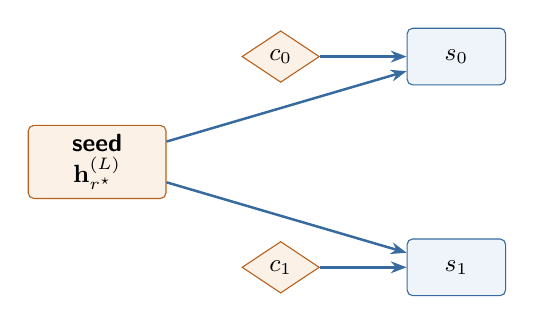
\begin{tikzpicture}[node distance=.65cm]
        \node[seed] (s) {seed\\$\mathbf h_{r^\star}^{(L)}$};
        \node[cand,above right=.7cm and 1.2cm of s] (c0) {$c_0$};
        \node[cand,below right=.7cm and 1.2cm of s] (c1) {$c_1$};
        \node[row,right=1.1cm of c0,minimum width=1.25cm] (o0) {$s_0$};
        \node[row,right=1.1cm of c1,minimum width=1.25cm] (o1) {$s_1$};
        \draw[fk] (s) -- (o0);
        \draw[fk] (c0) -- (o0);
        \draw[fk] (s) -- (o1);
        \draw[fk] (c1) -- (o1);
      \end{tikzpicture}
  \end{columns}
\end{frame}

% -----------------------------------------------------------------------------
% 16. Standard results
% -----------------------------------------------------------------------------
\begin{frame}{Standard classification performance}
  \begin{columns}[T,onlytextwidth]
    \column{.59\textwidth}
      \vspace{0pt}
      \begin{block}{Published Standard setting}
        \renewcommand{\arraystretch}{1.25}
        \begin{tabularx}{\linewidth}{Xrr}
          \toprule
          Model & Params & Macro AUROC $\times100$ \\
          \midrule
          Entity Mean & 0 & 66.7 \\
          Griffin(published) & 22.80M & 64.0 \\
          RT(published) & 22.30M & 69.7 \\
          RT(local) & 22.30M & \good{69.9} \\
          RowGraph-Base & \good{2.05M} & 67.6 \\
          \rowcolor{PaleOrange}RelGraph & 2.78M & 69.7 \\
          \bottomrule
        \end{tabularx}
      \end{block}

    \column{.37\textwidth}
      \vspace{0pt}
      \begin{alertblock}{Compact, not merely smaller}
        \centering
        {\fontsize{20}{22}\selectfont\bfseries\color{Orange}8.0$\times$}\par
        fewer trainable parameters than RT
      \end{alertblock}
      \vspace{.2cm}
      \begin{block}{Controlled gain}
        \centering
        Base $67.6$ $\rightarrow$ RelGraph $69.7$\\
        \good{$+2.1$ AUROC points}
      \end{block}
  \end{columns}
  \source{Entity Mean, Griffin, and RT use published Standard results; Base and RelGraph use our local full-test evaluations. Published Griffin/RT counts are rounded to 22M; the 8.0$\times$ ratio uses RT's exact 22.3M implementation count. Equal displayed means are not a significance claim}
\end{frame}


% % -----------------------------------------------------------------------------
% % 17. Relation conditioning ablation
% % -----------------------------------------------------------------------------
% \begin{frame}{Relation conditioning: controlled ablation}
%   \begin{columns}[T,onlytextwidth]
%     \column{.47\textwidth}
%       \vspace{0pt}
%       \begin{exampleblock}{Supported by the controlled ablation}
%         Adding the relation branch while holding the row backbone fixed:
%         \[
%           67.6\;\longrightarrow\;69.7
%           \qquad({\color{Green}\mathbf{+2.1}}\ \text{Standard}).
%         \]
%         Largest Standard gains:
%         \begin{itemize}
%           \item Avito User Clicks: $+7.3$
%           \item Stack User Engagement: $+6.3$
%           \item F1 Driver DNF: $+4.5$
%         \end{itemize}
%       \end{exampleblock}

%     \column{.47\textwidth}
%       \vspace{0pt}
%       \begin{alertblock}{Not supported as a universal claim}
%         NSL macro changes in the opposite direction:
%         \[
%           63.9\;\longrightarrow\;62.3
%           \qquad({\color{Red}\mathbf{-1.6}}\ \text{NSL}).
%         \]
%         Therefore:
%         \begin{itemize}
%           \item row-level construction supplies much of the robustness;
%           \item relation conditioning primarily improves Standard accuracy;
%           \item its NSL effect is heterogeneous across tasks.
%         \end{itemize}
%       \end{alertblock}
%   \end{columns}
% \end{frame}

% % -----------------------------------------------------------------------------
% % 18. Takeaways
% % -----------------------------------------------------------------------------
% \begin{frame}{Takeaways}
%   \begin{columns}[T,onlytextwidth]
%     \column{.32\textwidth}
%       \vspace{0pt}
%       \contentcard{GapOneTitle}{GapOneBody}
%         {Diagnose}
%         {RT can access historical target values in one column-attention step, creating a strong shortcut.}
%     \column{.32\textwidth}
%       \vspace{0pt}
%       \contentcard{GapTwoTitle}{GapTwoBody}
%         {Redesign}
%         {Pool cells into rows, then reason over explicit row and schema-relation graphs.}
%     \column{.32\textwidth}
%       \vspace{0pt}
%       \contentcard{GapThreeTitle}{GapThreeBody}
%         {Result}
%         {RelGraph matches published RT with 87.5\% fewer parameters; Base best preserves NSL performance.}
%   \end{columns}

%   \vspace{.48cm}
%   \begin{beamercolorbox}[sep=.62em,wd=\linewidth]{block body}
%     \centering
%     \normalsize\bfseries
%     The key shift is from \color{Red}cell-level shortcut access\color{Ink}\ to \color{Teal}explicit row- and relation-level reasoning\color{Ink}.
%   \end{beamercolorbox}

%   \vspace{.35cm}
%   \centering\small\color{Muted}
%   Next evidence needed: multi-seed uncertainty, frozen-context NSL, finalized regression, and measured runtime/memory.
% \end{frame}

% -----------------------------------------------------------------------------
% 17. Full task-level classification results
% -----------------------------------------------------------------------------
\begin{frame}{Full classification results}
  \centering
  \vspace{.10cm}
  \fontsize{8.3}{9.7}\selectfont
  \renewcommand{\arraystretch}{1.18}
  \setlength{\tabcolsep}{5.2pt}
  \begin{tabular}{lrrr@{\hspace{.55cm}}rrr}
    \toprule
    & \multicolumn{3}{c}{\bfseries\color{Blue}Standard context}
    & \multicolumn{3}{c}{\bfseries\color{Orange}NSL context} \\
    \cmidrule(lr){2-4}\cmidrule(lr){5-7}
    Task & RT(local) & Base & RelGraph & RT(local) & Base & RelGraph \\
    \midrule
    Amazon Item Churn
      & \cellcolor{PaleTeal}\good{70.2} & 68.4 & 66.9
      & 51.8 & \cellcolor{PaleTeal}\good{71.1} & 65.1 \\
    \rowcolor{PaleBlue}Amazon User Churn
      & \cellcolor{PaleTeal}\good{64.6} & 63.1 & 63.7
      & 54.9 & 61.5 & \cellcolor{PaleTeal}\good{61.8} \\
    Avito User Clicks
      & 58.5 & 53.8 & \cellcolor{PaleTeal}\good{61.1}
      & 53.9 & 59.5 & \cellcolor{PaleTeal}\good{61.2} \\
    \rowcolor{PaleBlue}Avito User Visits
      & 62.1 & 61.2 & \cellcolor{PaleTeal}\good{62.4}
      & 48.0 & 61.2 & \cellcolor{PaleTeal}\good{62.1} \\
    F1 Driver DNF
      & 79.1 & 75.3 & \cellcolor{PaleTeal}\good{79.7}
      & 69.7 & 46.4 & \cellcolor{PaleTeal}\good{70.8} \\
    \rowcolor{PaleBlue}F1 Driver Top-3
      & 89.1 & 88.0 & \cellcolor{PaleTeal}\good{89.6}
      & 46.3 & \cellcolor{PaleTeal}\good{87.1} & 67.0 \\
    H\&M User Churn
      & 64.2 & \cellcolor{PaleTeal}\good{67.2} & 66.8
      & 39.6 & 61.1 & \cellcolor{PaleTeal}\good{63.6} \\
    \rowcolor{PaleBlue}Stack User Badge
      & \cellcolor{PaleTeal}\good{80.6} & 75.1 & 76.8
      & 54.3 & \cellcolor{PaleTeal}\good{73.1} & 65.6 \\
    Stack User Engagement
      & \cellcolor{PaleTeal}\good{78.3} & 70.0 & 76.3
      & 49.9 & \cellcolor{PaleTeal}\good{64.0} & 52.9 \\
    \rowcolor{PaleBlue}Trial Study Outcome
      & 52.4 & \cellcolor{PaleTeal}\good{53.6} & 53.2
      & 52.4 & \cellcolor{PaleTeal}\good{53.6} & 53.2 \\
    \midrule
    \rowcolor{PaleOrange}\bfseries Macro average
      & \cellcolor{PaleTeal}\good{69.9} & 67.6 & 69.7
      & 52.1 & \cellcolor{PaleTeal}\good{63.9} & 62.3 \\
    \bottomrule
  \end{tabular}

  \vspace{.22cm}
  \begin{beamercolorbox}[sep=.42em,wd=.82\linewidth]{block body}
    \centering\scriptsize
    \colorbox{PaleTeal}{\strut\good{Green cells}} mark the best model within each three-column context group.
  \end{beamercolorbox}
  \source{Paired local full-test evaluations. RT Standard values on this page come from the locally evaluated checkpoint, not RT's published Table~1.}
\end{frame}



% -----------------------------------------------------------------------------
% 18. NSL results
% -----------------------------------------------------------------------------
\begin{frame}{Robustness without self-labels}
  \begin{columns}[T,onlytextwidth]
    \column{.58\textwidth}
      \vspace{0pt}
      \begin{block}{Paired macro comparison}
        \renewcommand{\arraystretch}{1.35}
        \begin{tabularx}{\linewidth}{Xrrr}
          \toprule
          Model & Standard & NSL & Drop $\downarrow$ \\
          \midrule
          RT (local) & 69.9 & 52.1 & \bad{17.8} \\
          \rowcolor{PaleTeal}RowGraph-Base & 67.6 & \good{63.9} & \good{3.7} \\
          RelGraph & 69.7 & 62.3 & 7.3 \\
          \bottomrule
        \end{tabularx}
      \end{block}

    \column{.38\textwidth}
      \vspace{0pt}
      \begin{exampleblock}{What this supports}
         Under the evaluated protocols, both row-graph models retain substantially more performance after self-label removal than RT.
      \end{exampleblock}
      \vspace{.18cm}
      % \begin{alertblock}{Natural control}
      %   Trial Study Outcome has no removable self-labels; Standard and NSL remain unchanged for all local models.
      % \end{alertblock}
  \end{columns}
  \source{Macro average over 10 classification tasks. NSL is a stress test, not a frozen-context causal intervention.}
\end{frame}


% -----------------------------------------------------------------------------
% 19. Future work
% -----------------------------------------------------------------------------
\begin{frame}{Future work}
  \vspace{.55cm}
  \centering
  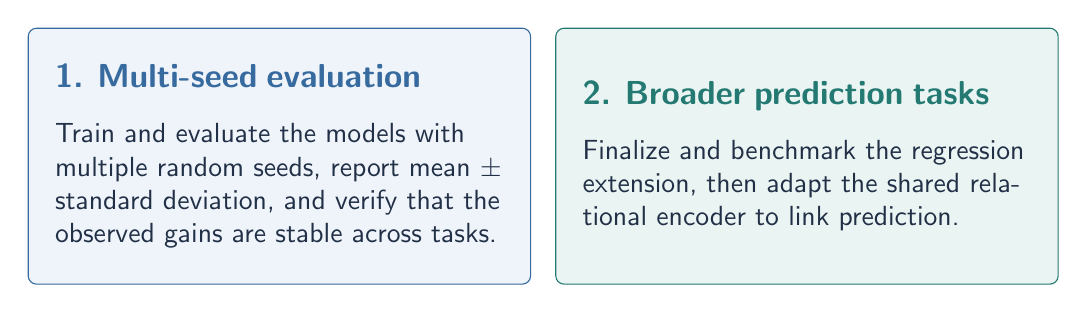
\begin{tikzpicture}
    \node[anchor=north,draw=Blue,fill=PaleBlue,rounded corners=3pt,
          text width=5.70cm,minimum height=3.25cm,inner sep=.34cm,align=left] (seeds) at (-3.35,0) {%
      {\large\bfseries\color{Blue}1. Multi-seed evaluation}\\[.28cm]
      {\normalsize\color{Ink}Train and evaluate the models with multiple random seeds, report mean $\pm$ standard deviation, and verify that the observed gains are stable across tasks.}};

    \node[anchor=north,draw=Teal,fill=PaleTeal,rounded corners=3pt,
          text width=5.70cm,minimum height=3.25cm,inner sep=.34cm,align=left] (tasks) at (3.35,0) {%
      {\large\bfseries\color{Teal}2. Broader prediction tasks}\\[.28cm]
      {\normalsize\color{Ink}Finalize and benchmark the regression extension, then adapt the shared relational encoder to link prediction.}};
  \end{tikzpicture}

  \vspace{.65cm}
  \begin{beamercolorbox}[sep=.58em,wd=.90\linewidth]{block body}
    \centering\bfseries
    Goal: establish reproducible performance and a task-general relational backbone.
  \end{beamercolorbox}
\end{frame} 
\end{document}
